\documentclass[a4paper,11pt]{exam}
\usepackage[utf8]{inputenc}
\usepackage{enumerate}

%\usepackage{lipsum}

\date{12 November 2018}
\title{RE355 - Introduction to Cloud Networking\\
Lab session 4: Advanced issues in cloud computing}
\author{Simon Da Silva \and Mathias Lacaud}

%\usepackage{fancyhdr}
\usepackage{listings}
\usepackage{graphicx}

%\pagestyle{fancy}
%\fancyhf{}
\rhead{Bordeaux INP: ENSEIRB-MATMECA}
\lhead{RE355 - Introduction to Cloud Networking}

\lstset{language=sh,basicstyle=\ttfamily,columns=fullflexible}
\begin{document}

\maketitle

\section{Introduction - Setup}

This lab session deals with the use of Docker Swarm and additional tools to discover the issues with file sharing and elasticity in distributed systems. 
As it is the final lab session, you are supposed to know the basics.
We will expect you to search and find information by yourselves in the official documentations.
For this session, you need to work in groups with 3 to 4 computers on the same local network.

First of all, reinitialize each computer:

\begin{lstlisting}[frame=single,language={sh}]  % Start your code-block

$ razrezo

$ date --set "$(curl https://time.akamai.com/?iso)"

$ docker service restart 

\end{lstlisting}

Be sure that chromium is installed in at least one of your computers: 

\begin{lstlisting}[frame=single,language={sh}]  % Start your code-block

$ apt install chromium
	
\end{lstlisting}

You can start chromium as root in a terminal by using: 

\begin{lstlisting}[frame=single,language={sh}]  % Start your code-block

$ chromium --no-sandbox &
		
\end{lstlisting}

Then, create your swarm with: 

\begin{lstlisting}[frame=single,language={sh}]  % Start your code-block

$ docker swarm init

\end{lstlisting}

and join the swarm with all the machines.

Download the correction of the 2nd lab session from Moodle and extract it. 
Go into the extracted folder, modify the published port of the frontend service and expose the port 80.Once done, start the application:

\begin{lstlisting}[frame=single,language={sh}]  % Start your code-block

$ docker stack deploy --compose-file docker-compose.yml {stack-name}

\end{lstlisting}

After a few seconds, you should be able to see your running application at the address \textbf{http://127.0.0.1:3000/} in chromium:

\begin{lstlisting}[frame=single,language={sh}]  % Start your code-block

$ chromium --no-sandbox http://127.0.0.1/ &
		
\end{lstlisting}

\clearpage

\section{File systems in the application}

Two application modules (inside containers) are storing informations on their local file system. 
The \textbf{Server} is storing the raw video waiting to be encoded, and the encoded video to be served, in its folder \textit{/go/app/fileServers}. 
The \textbf{Storage} (i.e. the database) is storing data in its folder \textit{/var/lib/mysql}. 

\begin{figure}[!ht]
	\centering
	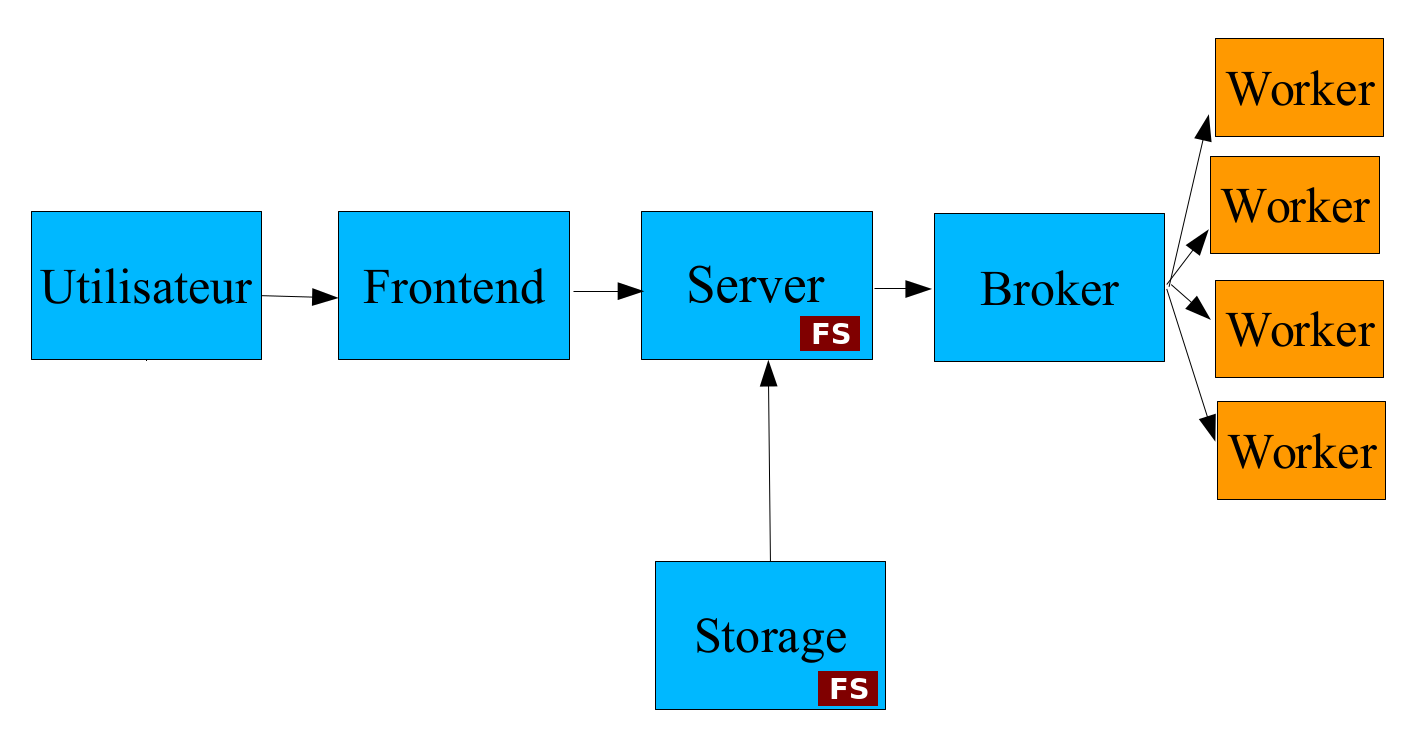
\includegraphics[width=0.8\textwidth]{fig/architecture.png}
	\label{fig:architecture}
\end{figure}

\section{The problem with volumes...}

This section introduces the problem of volumes in Docker.

\subsection{Safe replication}

\begin{questions}
	\question Using \textbf{docker service}, create 3 replicas of the frontend.
	\begin{enumerate}[(a)]
		\item Refresh the web page several times. Do you see any change in the page? Does the application still work from different Frontend containers?
		\item Why is the replication of the Frontend working?
	\end{enumerate}
\end{questions}

\subsection{Critical replication}

\begin{questions}
	\question Using \textbf{docker service}, create 3 replicas of the server.
	\begin{enumerate}[(a)]
		\item Refresh the web page several times. Is the application still working every time?
		\item Knowing that the video data are stored on the file system of the server, what is happening?
		\item Docker Swarm does not include any tool to create distributed volumes. Do you know any tool to create distributed file systems?
	\end{enumerate}
\end{questions}

\subsection{Persistence in the database}

\begin{questions}
	\question Using \textbf{docker service}, create 3 replicas of the database.
	\begin{enumerate}[(a)]
		\item Refresh the web page several times. Is the application still working every time?
		\item Why?
	\end{enumerate}
\end{questions}

\clearpage

\section{Network file system}

\subsection{NFS Server}

As Docker Swarm and many orchestrators do not have embedded solution for volume management across the nodes, it should be handled by the user.
This section is about the creation of a distributed file system simultaneously mounted on every computers of the cluster using \textbf{NFS} (as a simple example).

First of all, install NFS:

\begin{lstlisting}[frame=single,language={sh}]  % Start your code-block

$ apt install nfs-kernel-server
			
\end{lstlisting}

Modify the file /etc/exports and export 2 folders of the server.

\begin{lstlisting}[frame=single,language={sh}]  % Start your code-block

/nfs_server *(rw,sync,fsid=0,no_root_squash,subtree_check)
/nfs_database *(rw,sync,fsid=0,no_root_squash,subtree_check)	
			
\end{lstlisting}

Start the nfs and rpcbind service: 

\begin{lstlisting}[frame=single,language={sh}]  % Start your code-block

service nfs-server start	
service rpcbind start			

\end{lstlisting}

\subsection{Volume mounted on the nodes}

\begin{questions}
	\question Mount the file system on the other computers.
	\begin{enumerate}[(a)]
		\item What command do you use?
		\item How can you test if the distributed file system is working?
	\end{enumerate}
	\question Bind the volumes to the server and database service in the \textit{docker-compose.yml} file.
	\begin{enumerate}[(a)]
		\item What lines did you add?
		\item Is the application fully functional when the server is replicated now?
	\end{enumerate}
\end{questions}

\subsection{Volume mounted on the services}

\begin{questions}
	\question In the \textit{docker-compose.yml} file, create a docker volume connected with the nfs-server. 
You can use the official documentation\footnote{https://docs.docker.com/engine/reference/commandline/volume/}.
	\begin{enumerate}[(a)]
		\item What did you add in the docker-compose.yml file?
		\item What is the difference with the previous solution?
	\end{enumerate}
	\question Bind the volumes on the server and database service in the \textit{docker-compose.yml}.
	\begin{enumerate}[(a)]
		\item What lines did you add?
		\item Is the application fully functional when the server is replicated now?
	\end{enumerate}
\end{questions}

\clearpage

\section{Monitoring}
\subsection{Monitoring tools and manual scalling}
This section deals with the monitoring of the cluster. The goal is to get the metrics of CPU, RAM and Bandwidth usage of the computers in our cluster.

We are going to install some interesting monitoring tools like Prometheus, node-exporter, cAdvisor and Grafana. 
Those tools are very powerful but can be hard to install, understand and configure.
In order to simplify the process and see the basics, we are going to use a starter kit with a working docker compose file.

Download the source code from:
\begin{lstlisting}[frame=single,language={sh}]  % Start your code-block

$ curl https://github.com/stefanprodan/swarmprom/archive/master.zip >  \
swarmprom.zip
\end{lstlisting}

On the manager node, deploy the stack using: 
\begin{lstlisting}[frame=single,language={sh}]  % Start your code-block

$ cd swarmprom
$ ADMIN_USER=admin \
 ADMIN_PASSWORD=admin \
 docker stack deploy -c docker-compose.yml monitoring
\end{lstlisting}

\begin{questions}
	\question Explain quickly with your own words:
	\begin{enumerate}[(a)]
		\item What is cAdvisor?
		\item What is node-exporter?
		\item What is Prometheus?
		\item What is Grafana?
	\end{enumerate}
	\question Go to \textbf{http://127.0.0.1:3000/} to see the Grafana interface.
	\begin{enumerate}[(a)]
		\item What type of informations do you have access to?
	\end{enumerate}
	\question Start a video transcoding from the frontend.
	\begin{enumerate}[(a)]
		\item Discuss the CPU usage. Can you know on which computer the video is transcoded?
		\item Discuss the other metrics.
	\end{enumerate}

	\question Start several video transcoding from the frontend.
	\begin{enumerate}[(a)]
		\item What do you see?  
		\item Scale the worker up to 3 replicas. What do you see now? Discuss the parallelization of the transcoding.
	\end{enumerate}
\end{questions}


\section{Automatic scalling}

Pistes: rabbitmq-management, prometheus, docker stats

\end{document}
